\section{Unions}
\begin{itemize}
    \item Unions are used to combine the results of several select statements into one.
    \item Return the first name of the employees and the branches:
        \begin{minted}[autogobble]{sql}
            SELECT first_name FROM employee UNION
            SELECT branch_name FROM branch;
        \end{minted}
        \begin{figure}[H]
            \centering
            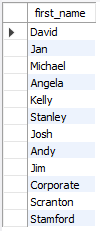
\includegraphics[width=0.4\textwidth]{./Figs/2020-12-24-21-02-55.png}
        % 	\caption{}
        \end{figure}
    
    \item When using unions the number of columns selected in each select statement needs to be the same in terms of quantity:
        \begin{minted}[autogobble]{sql}
            SELECT first_name, last_name FROM employee UNION
            SELECT branch_name FROM branch;-- error
        \end{minted}
        \begin{figure}[H]
            \centering
            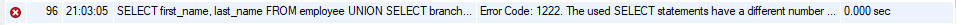
\includegraphics[width=0.4\textwidth]{./Figs/2020-12-24-21-03-18.png}
        % 	\caption{}
        \end{figure}
    
    \item They need to be of similar data types.
    \item The union can be performed with lots of select statements:
        \begin{minted}[autogobble]{sql}
            SELECT first_name FROM employee UNION
            SELECT branch_name FROM branch UNION
            SELECT client_name FROM client;
        \end{minted}
        \begin{figure}[H]
            \centering
            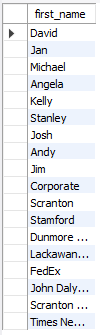
\includegraphics[width=0.4\textwidth]{./Figs/2020-12-24-21-03-42.png}
        % 	\caption{}
        \end{figure}
    
    \item Find a list of all clients and branch suppliers' names:
        \begin{minted}[autogobble]{sql}
            SELECT client_name FROM client UNION 
            SELECT supplier_name FROM branch_supplier;
        \end{minted}
        \begin{figure}[H]
            \centering
            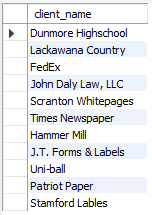
\includegraphics[width=0.4\textwidth]{./Figs/2020-12-24-21-04-04.png}
        % 	\caption{}
        \end{figure}

    \item Find a list of all money spent or earned by the company:
        \begin{minted}[autogobble]{sql}
            SELECT salary FROM employee UNION 
            SELECT total_sales FROM works_with;
        \end{minted}
        \begin{figure}[H]
            \centering
            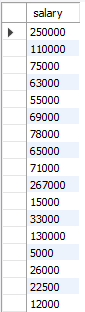
\includegraphics[width=0.4\textwidth]{./Figs/2020-12-24-21-04-28.png}
        % 	\caption{}
        \end{figure}
\end{itemize}
